\section{Maschinelles Lernen} \label{chpt:Stand_der_Technik_Maschinelles_Lernen}
Ein Teilgebiet der künstlichen Intelligenzen ist der Bereich des Maschinellen Lernens, welcher die Verarbeitung von Daten addressiert, um beispielsweise Vorhersagen in Situationen auf Basis von bestimmten Informationen zu treffen.
Im Jahr 1959 wurde dieser von Arthur Samuel geprägt, der die Herausforderung annahm, ein Schachspiel mit Hilfe einer Maschine zu lösen (\cite[4]{joshi_machine_2020}).
Das besondere hierbei ist das Erlernen des richtigen Lösungswegs, welcher nicht durch bestimmte Bedingungen gesteuert, sondern auf Basis verschiedener Informationen erlernt wird, die über diverse Quellen beigefügt werden.
Maschinelles Lernen findet in vielen Bereichen Anwendung, von Spracherkennung, Bilderkennung bis hin zu selbstfahrenden Kraftfahrzeugen. Diese Technologie wird zunehmend wichtiger in unserer stetig vernetzteren Welt und trägt dazu bei, komplexer werdende Probleme zu lösen und immer innovativere Lösungen in verschiedenen Branchen zu entwickeln.

Im Wesentlichen geht es um die Entwicklung von Algorithmen, die dem Computer das Erkennen von Mustern und Zusammenhängen in Daten ermöglichen, wordurch ohne menschliche Intervention Aufgaben erledigt werden können.
Daher trainiert man Algorithmen auf Basis großer Datenbestände, wodurch das jeweilige Modell so generalisiert wie möglich angepasst wird, sodass die erlernten Fähigkeiten auf neu erhobene Daten angewendet werden können. Das Erlernen des nötigen Wissens basiert hierbei auf drei wesentlichen Faktoren, die die Qualität des Trainings beeinflussen. Neben den Informationen, die aus Daten gewonnen werden, nutzt man eine Kennzahl, die einen Vergleich zwischen dem aktuellen und idealen Verhalten herstellt, um mit dem dritten Faktor - einem Rückkopplungsmechanismus - das Programm anzuleiten eine verbesserte Leistung in Folgeergebnissen zu erzielen (\cite[4]{joshi_machine_2020}).

Um ein Modell trainieren zu können, wird ein geeignetes maschinelles Lernverfahren ausgewählt, das darauf abzielt, die Ausgaben eines KI-Systems in Bezug auf bestimmte Systemeingaben im Laufe des Lernprozesses zu optimieren. Unterschieden wird hautpsächlich in der Art und Weise, wie die \glqq Kritik\grqq{} präsentiert wird, die zur Verbesserung des Verhaltens der jeweiligen künstlichen Systeme führen soll. Ein Training basiert auf sogenannten Hyperparametern, die Rahmenbedingungen des Prozesses festlegen. Dies kann zum Beispiel die Anzahl der Epochen, die Lern-Rate oder auch die Batch-Größe sein. Im Folgenden werden drei prägende Lernverfahren näher beschrieben.
\subsection{Überwachtes Lernen}\label{subsec:supervisedlearning}
Überwachtes Lernen (eng.: supervised learning) stellt einen wesentlichen Bereich des maschinellen Lernens dar, um aus Informationen, bestehend aus Datenpunkten \textit{$X = x_1, x_2, \ldots, x_n$} mit zugehörigem Label aus \textit{$Y = y_1, y_2, \ldots, x_n$}, das nötige Wissen für bestimmte Anwendungsfälle zu erlangen. Anwendung findet dieses Verfahren in Systemen, die einen bestimmten Input $I$ verarbeiten, um darauf basierend eine Vorhersage über das zugehörige Label abzugeben.
Mögliche Arten von neuronalen Netzwerken, die über diese Methode trainiert wurden, sind beispielsweise Bildklassifikatoren. Dabei ist es die Aufgabe des Modells $M$, basierend auf einem bestimmten Input $I$ mit Hilfe erlernter Muster und Zusammenhänge der Trainingsdaten eine Vorhersage über die Kategorie oder das Label von $I$ zu treffen.
\begin{figure}[H]
	\hspace{-30mm}
	\centering
	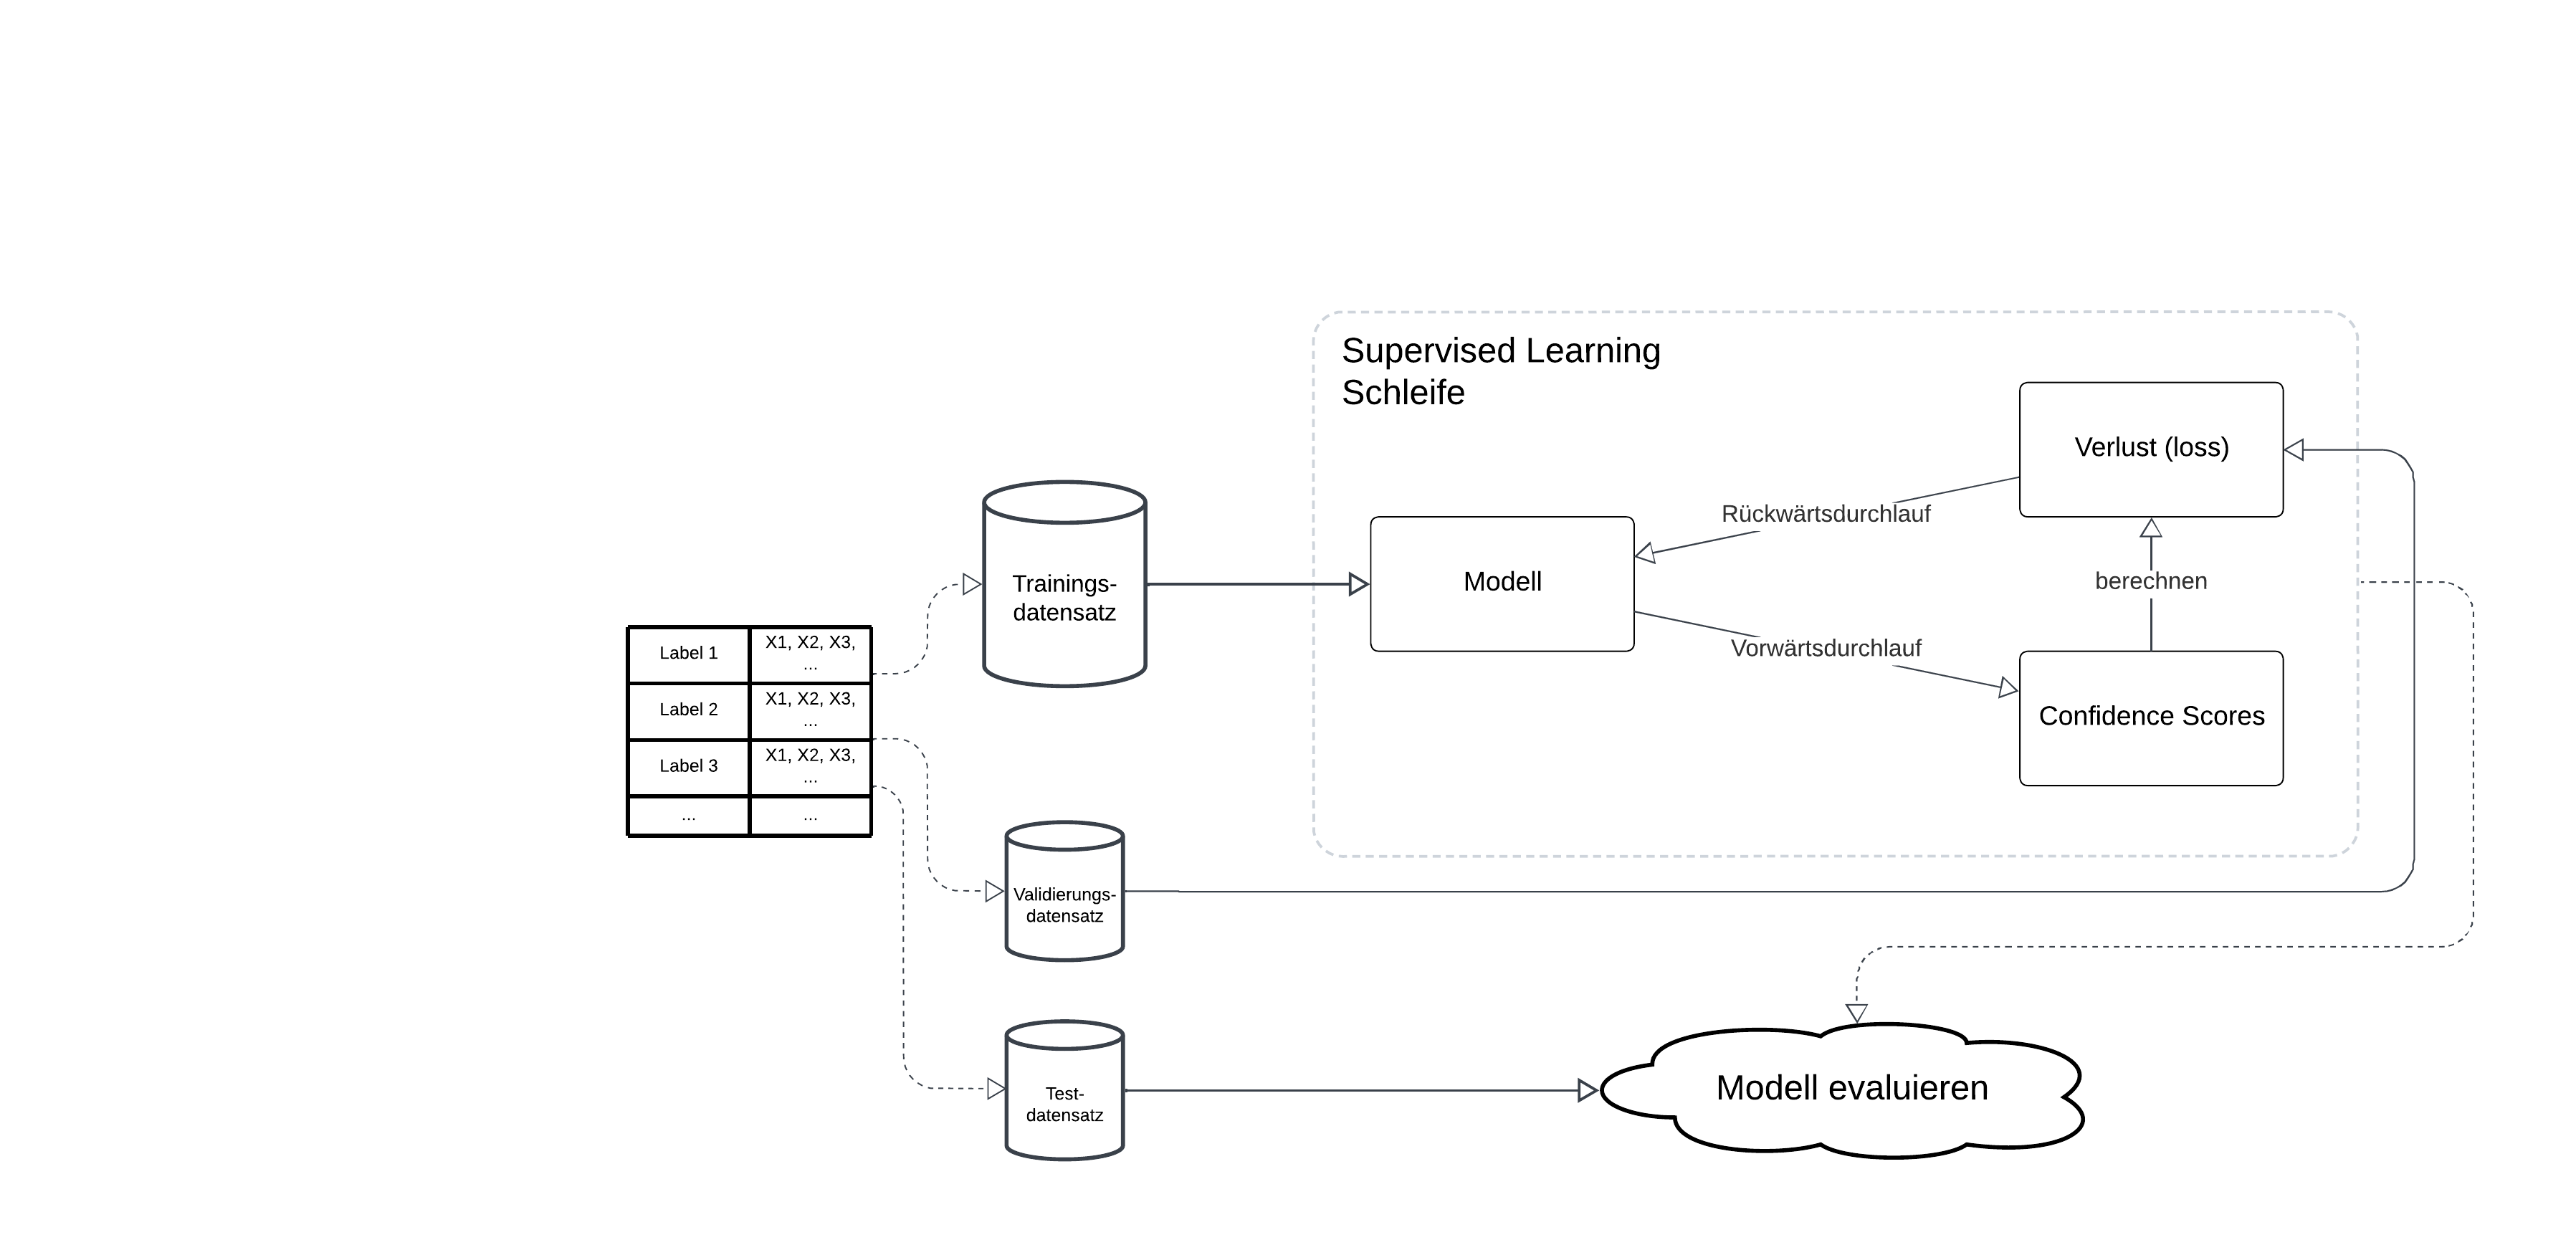
\includegraphics[width=\linewidth]{Bilder/SupervisedLearning.png}
	\caption{Prozessvisualisierung: überwachtes Lernen}
\end{figure}
Der \textit{Ablauf} des Trainings lässt sich wie folgt beschreiben: nach Beenden von Datensammlung, Datenvorverarbeitung und Datensatztrennung in einen Trainings-, Validierungs- und Testdatensatz beginnt der eigentliche Teil des Trainings, wobei die Trainings- und Validierungsdaten für die Aktualisierung der interenen Modelleinstellungen, wie Gewichtungen und Schwellenwerte, verwendet werden. Die Optimierung der Parameter wird auf Basis der Verlustfunktion mit Hilfe eines Rückwärtsdurchlaufes (eng.: Backward Propagation) durchgeführt, die mit der Differenz zwischen Vorhersagen des Modells aus dem Vorwärtsdurchlauf (eng.: Forward Propagation) und den realen Labeln berechnet wird.

Die \textit{Qualität} des Trainings wird meist anhand der Genauigkeit von Vorhersagen bestimmt, welche ausdrückt, wie gut die Klassifikation von im Training ungesehenen Daten funktioniert.
\begin{equation}
\text{Genauigkeit} = \frac{\text{Anzahl korrekter Vorhersagen}}{\text{Gesamtanzahl der Vorhersagen}}
\end{equation}
 Weitere Metriken können die Präzision (eng.: Precision), der Recall oder auch der F1-Score sein. Neben Messungen der Modell-Genauigkeit kann man die Qualität des trainierten Modells auch anhand der Verlustfunktion (eng.: loss-function) oder der \glqq Area Under the Curve\grqq{} (AUC), welche die Fläche unter der \glqq Receiver Operating Characteristic\grqq{} (ROC) -- dem Verhältnis zwischen der True- und False-Positive-Rate -- messen.
\subsection{Unüberwachtes Lernen}\label{subsec:unsupervisedlearning}
\begin{figure}[H]
	\centering
	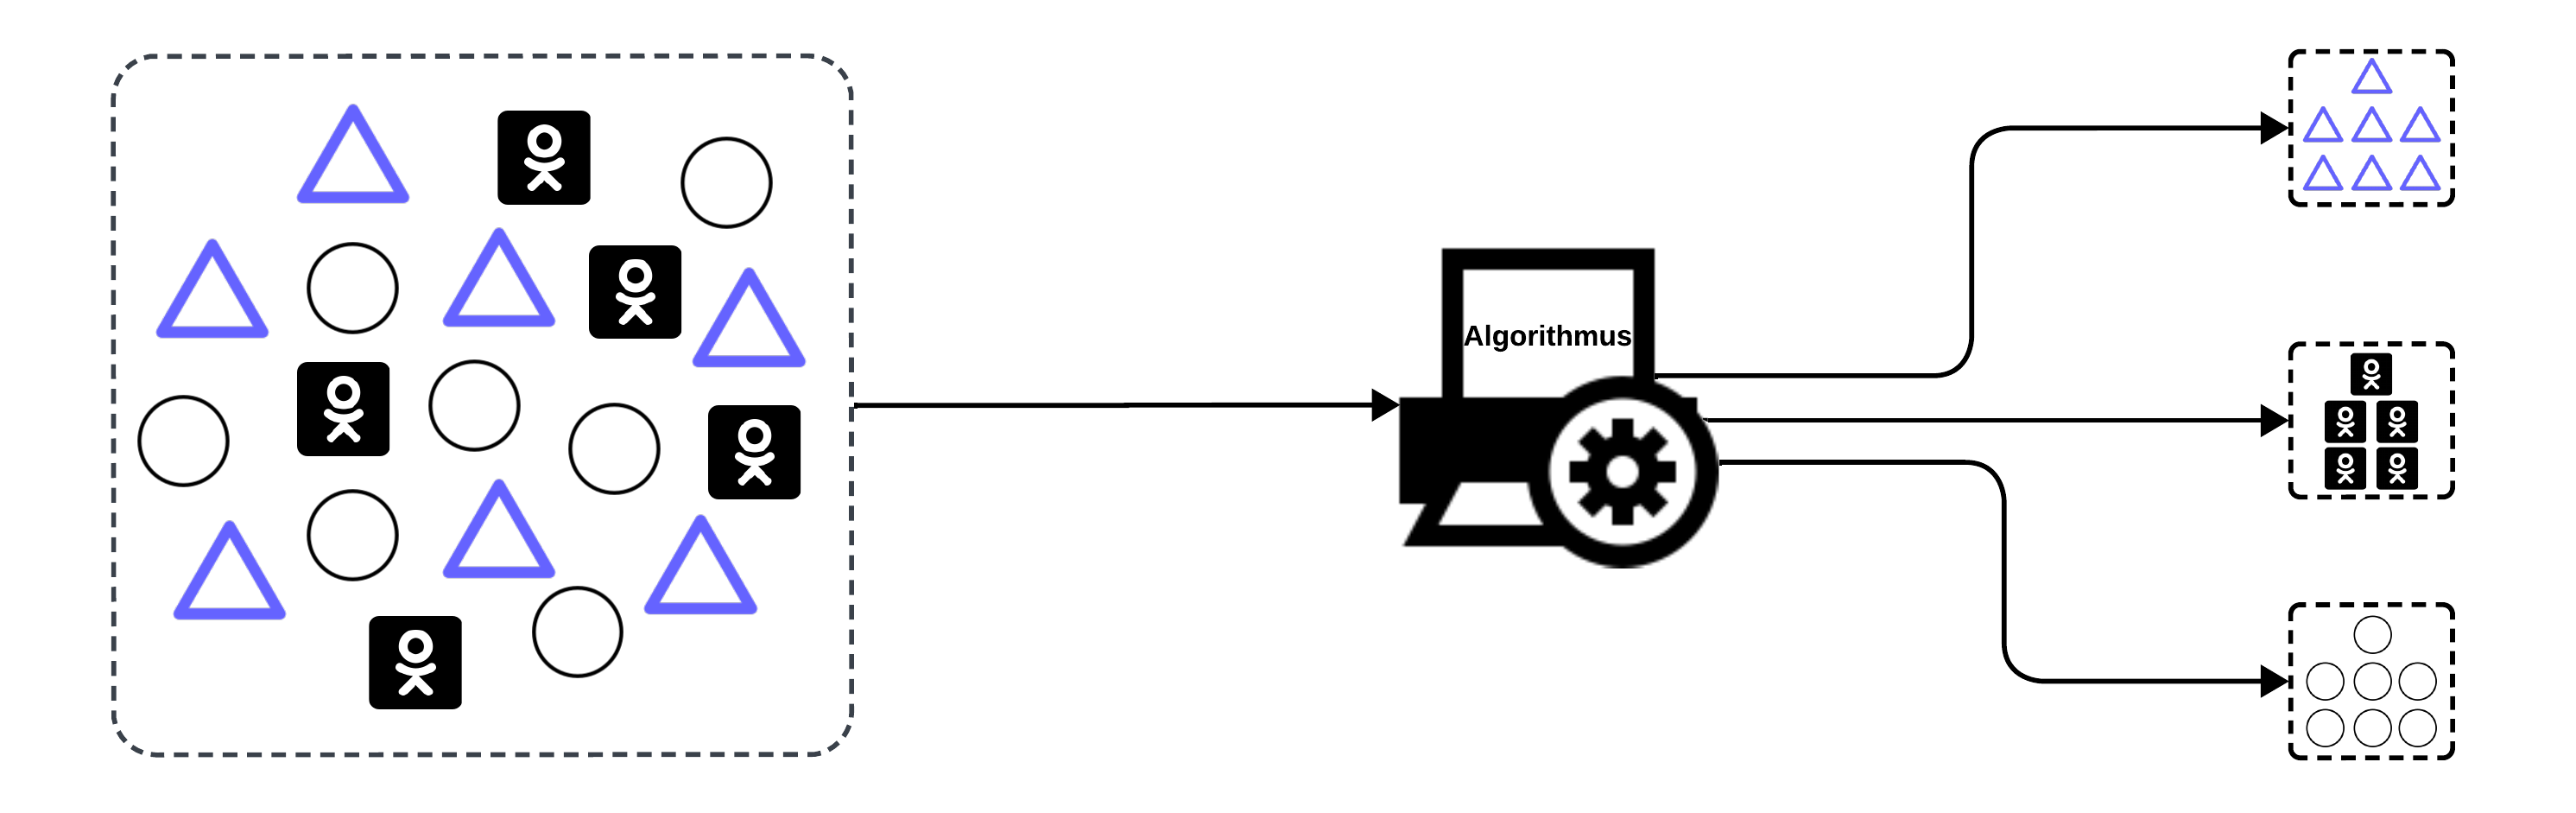
\includegraphics[width=0.8\linewidth]{Bilder/unsupervised_sample.png}
	\caption{Resultat eines auf unüberwachtem Lernen basierenden Clusterings}
\end{figure}
Unüberwachtes Lernen (eng.: unsupervised learning) stellt einen anderen bedeutenden Bereich im maschinellen Lernen dar, der sich von überwachtem Lernen (\ref{subsec:supervisedlearning}) dahingegen unterscheidet, dass keine expliziten Label/Kategorien für die Trainingsdaten bereitgestellt werden, weshalb das Aufteilen des Datensatzes in 3 unabhängige Teile nicht notwendig ist. Diese Methode wird angewendet, wenn das Ziel darin besteht, Muster, Strukturen oder Zusammenhänge in den Daten zu finden, ohne dabei Kategorien oder Label vorzugeben. Dabei wird basierend auf Informationen eines Datensatzes, bestehend aus Datenpunkten \textit{$X = x_1, x_2, \ldots, x_n$}, trainiert. \glqq Aufgabe ist es hier, passende Repräsentationen zu finden, die beispielsweise die Erkennung von Charakteristika in Datenmengen, Wiedererkennung von Ausnahmen oder die Erstellung von Prognosen ermöglichen.\grqq (\cite[5]{lorenz_reinforcement_2020}) Im Gegensatz zu Überwachtem Lernen (\ref{subsec:supervisedlearning}) geht es nicht um das Zurdnen von Mustern in vorhandenen Kategorien, sondern um das Auffinden von zum Beispiel Clustern in einer bestimmten Datenmenge $X$. Dabei werden Modellparameter nicht über eine Verlustfunktion, die durch die Differenz zwischen tatsächlichem und vorhergesagtem Label berechnet wird, dargestellt, sondern die Parameter werden für die Repräsentation inhärenter Muster in den Daten angepasst. Für die Auswertung des Algorithmus trägt das Nutzen eines zusätzlichen Datensatzes für die Qualitätsbewertung bei.
\begin{figure}[H]\label{img:unsupervisedworkflow}
	\hspace{-15mm}
	\centering
	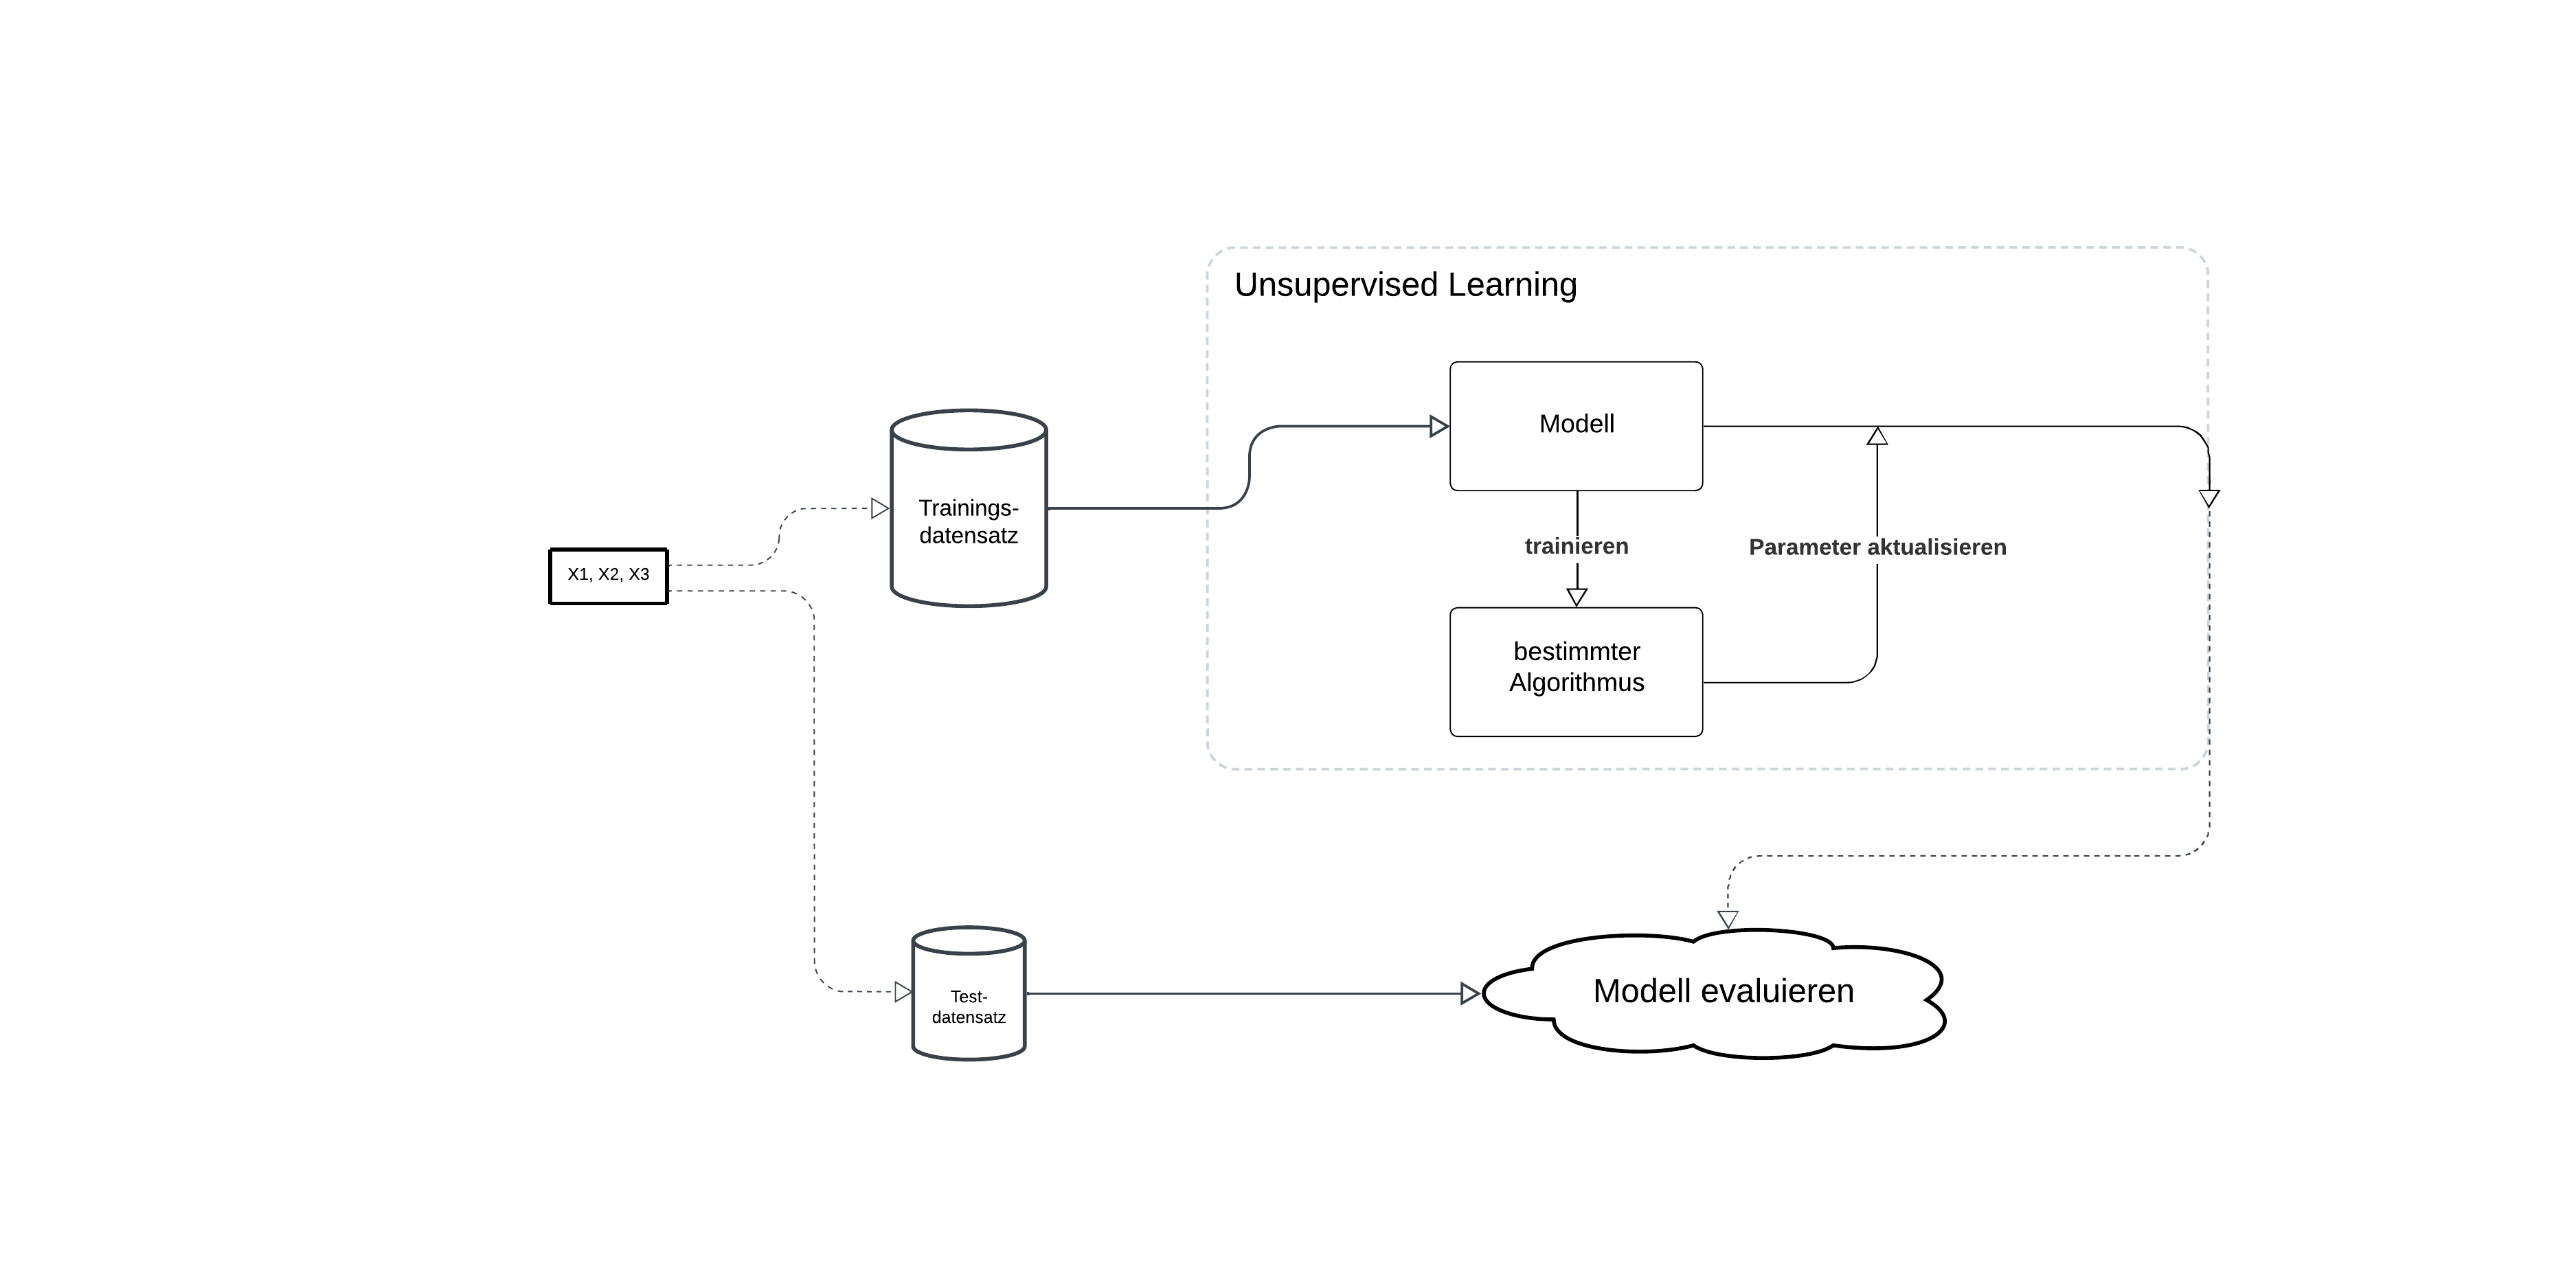
\includegraphics[width=\linewidth]{Bilder/UnsupervisedLearning.png}
	\caption{Prozessvisualisierung: unüberwachtes Lernen}
\end{figure}
Der \textit{Ablauf} des Trainigs gestaltet sich wie folgt: Nach Abschluss von Datensammlung und Vorverarbeitung beginnt der eigentliche Prozess des unüberwachten Lernens. Im Gegensatz zum überwachten Lernen (\ref{subsec:supervisedlearning}) gibt es hierbei keine vordefinierten Zielvariablen. Den Datenpunkten $X = x_1, x_2, \ldots, x_n$ ist also initial keine Kategorie beziehungsweise kein Label zugeordnet, da die Menge $Y$ bist dato nicht existent ist. Im Gegensatz zu überwachtem Lernen nutzt man hier Algorithmen wie beispielsweise \glqq $k$-Nearest Neighbors (KNN)\grqq{} (\cite[38]{joshi_machine_2020}), um eine bestimmte Operation auf den zu behandelnden Datensatz auszuführen. Mit Hilfe des Algorithmus wird ein bestimmtes Modell dahingehend trainiert, dass es einen Datensatz zum Beispiel in bestimmte Kategorien unterteilen kann. Dafür analysiert der Algorithmus die jeweiligen Datenpunkte und versucht diese mit Hilfe von Zusammenhängen und verschiedenen extrahierten Merkmalen zu interpretieren. Anhand des dabei erlangten Wissens werden Modellparameter aktualisiert, wonach das unüberwachte Lernen beendet ist. Ein Ergebnis kann hierbei beispielsweise ein \glqq geclusterter\grqq{} Datensatz sein.

Die  \textit{Qualität} eines Modells ist schwieriger zu messen als bei überwachtem Lernen, da keine klar definierte Zielvariable vorliegt, mit Hilfe welcher eine Genauigkeitsanalyse durchgeführt werden kann. Dennoch lässt sich ein auf unüberwachtem lernen basierter Clustering-Algorithmus mit verschiedenen Metriken evaluieren. Zum einen kann man den sogenannten Silhouette Score (\cite{shahapure_cluster_2020}) nutzen, da dieser das Zusammenpassen der verschiedenen Datenpunkte innerhalb eines Clusters bewertet. Je höher dieser Wert, desto besser sind die jeweiligen Cluster definiert. Neben Metriken, die durch bestimmte Berechnungen repräsentiert werden, lässt sich die Qualität eines Modells auch durch visuelle Methoden wie der Auswahl geeigneter Plots messen, die die Zugehörigkeit verschiedener Datenpunkte darstellen.
\subsection{Bestärkendes Lernen}
Das bestärkende Lernen (eng.: reinforcement learning) (\cite[S. 13 ff.]{lorenz_reinforcement_2020}) ist ein maschinelles Lernverfahren, das sich von überwachtem und unüberwachtem unterscheidet. Es basiert auf der Interaktion eines Agenten mit seiner Umgebung und ist auf Rückmeldungen dieser angewiesen. Im Gegensatz zu überwachten Lernverfahren gibt es keine vorgegebenen Label für die Datenpunkte, weshalb Reinforcement Learning nicht als vollständig überwacht betrachtet werden kann. Gleichzeitig fehlt es den Datenpunkten an der Strukturierung, die für unüberwachte Lernverfahren typisch ist. Die Interaktion mit der Umgebung erfolgt durch den Agenten, der verschiedene Erfahrungen sammelt, während dieser Aktionen ausführt. Das Hauptziel des Algorithmus besteht darin, den Agenten so zu trainieren, dass er in seiner spezifischen Umgebung optimale Aktionen durchführt, um eine maximale kumulative Belohung über die Dauer des Lernprozesses zu erzielen. Diese Belohnungen und Strafen werden von der Umgebung basierend auf den vom Agenten durchgeführten Aktionen übergeben. Damit der Agent das Ziel der maximalen kumulativen Belohnung erreicht, erfordert dies eine geschickte Balance zwischen der Erkundung neuer Aktionen und der Ausführung bekannter, belohnungsreicher Aktionen, wobei der Agent seine Strategie kontinuierlich anpassen und verbessern muss. Bestärkendes Lernen wird in diversen Anwendungen eingesetzt, wie beispielsweise in Spielstrategien, in autonom-fahrenden Kraftfahrzeugen oder im Bereich der Robotik. Das Lösen komplexer Aufgaben hat durch den Einsatz tiefer neuronaler Netzwerke im \glqq Deep Reinforcement Learning\grqq{}-Bereich zu bedeutendem Fortschritt geführt. Im Allgemeinen ist das bestärkende Lernen eine mächtige Methode, um intelligente Agenten für das Lösen komplexer Probleme in dynamischen Umgebungen zu trainieren. Diese sind dann in der Lage, optimale Entscheidungen zu treffen.

Zu den wichtigsten Bestandteilen des bestärkenden Lernverfahrens zählen neben dem Agenten und der Umgebung auch Belohnungen, Zustände, Zustandsübergänge und Aktionen. Die Teile des Verfahrens lassen sich in zwei Gruppen unterteilen: zum einen der Agent mit den jeweiligen Aktionen und die Umgebung, mit den Zuständen und Belohnungen. Diese Umgebung bestimmt die neuen Zustände anhand der Veränderung basierend auf die Aktion, welche vom Agenten ausgeführt wird. Ein Zustand beschreibt hier die genaue Konfiguration der Umgebung zu einem bestimmten Zeitpunkt $t$. Ein Beispiel für einen Zustand kann das aktuelle Schachbrett mit den Positionen der jeweiligen Figuren sein, die durch eine Aktion und dem damit zusammenhängenden Zustandsübergang verändert wurden.
\begin{figure}[H]\label{img:reinforcementworkflow}
	\hspace{-10mm}
	\centering
	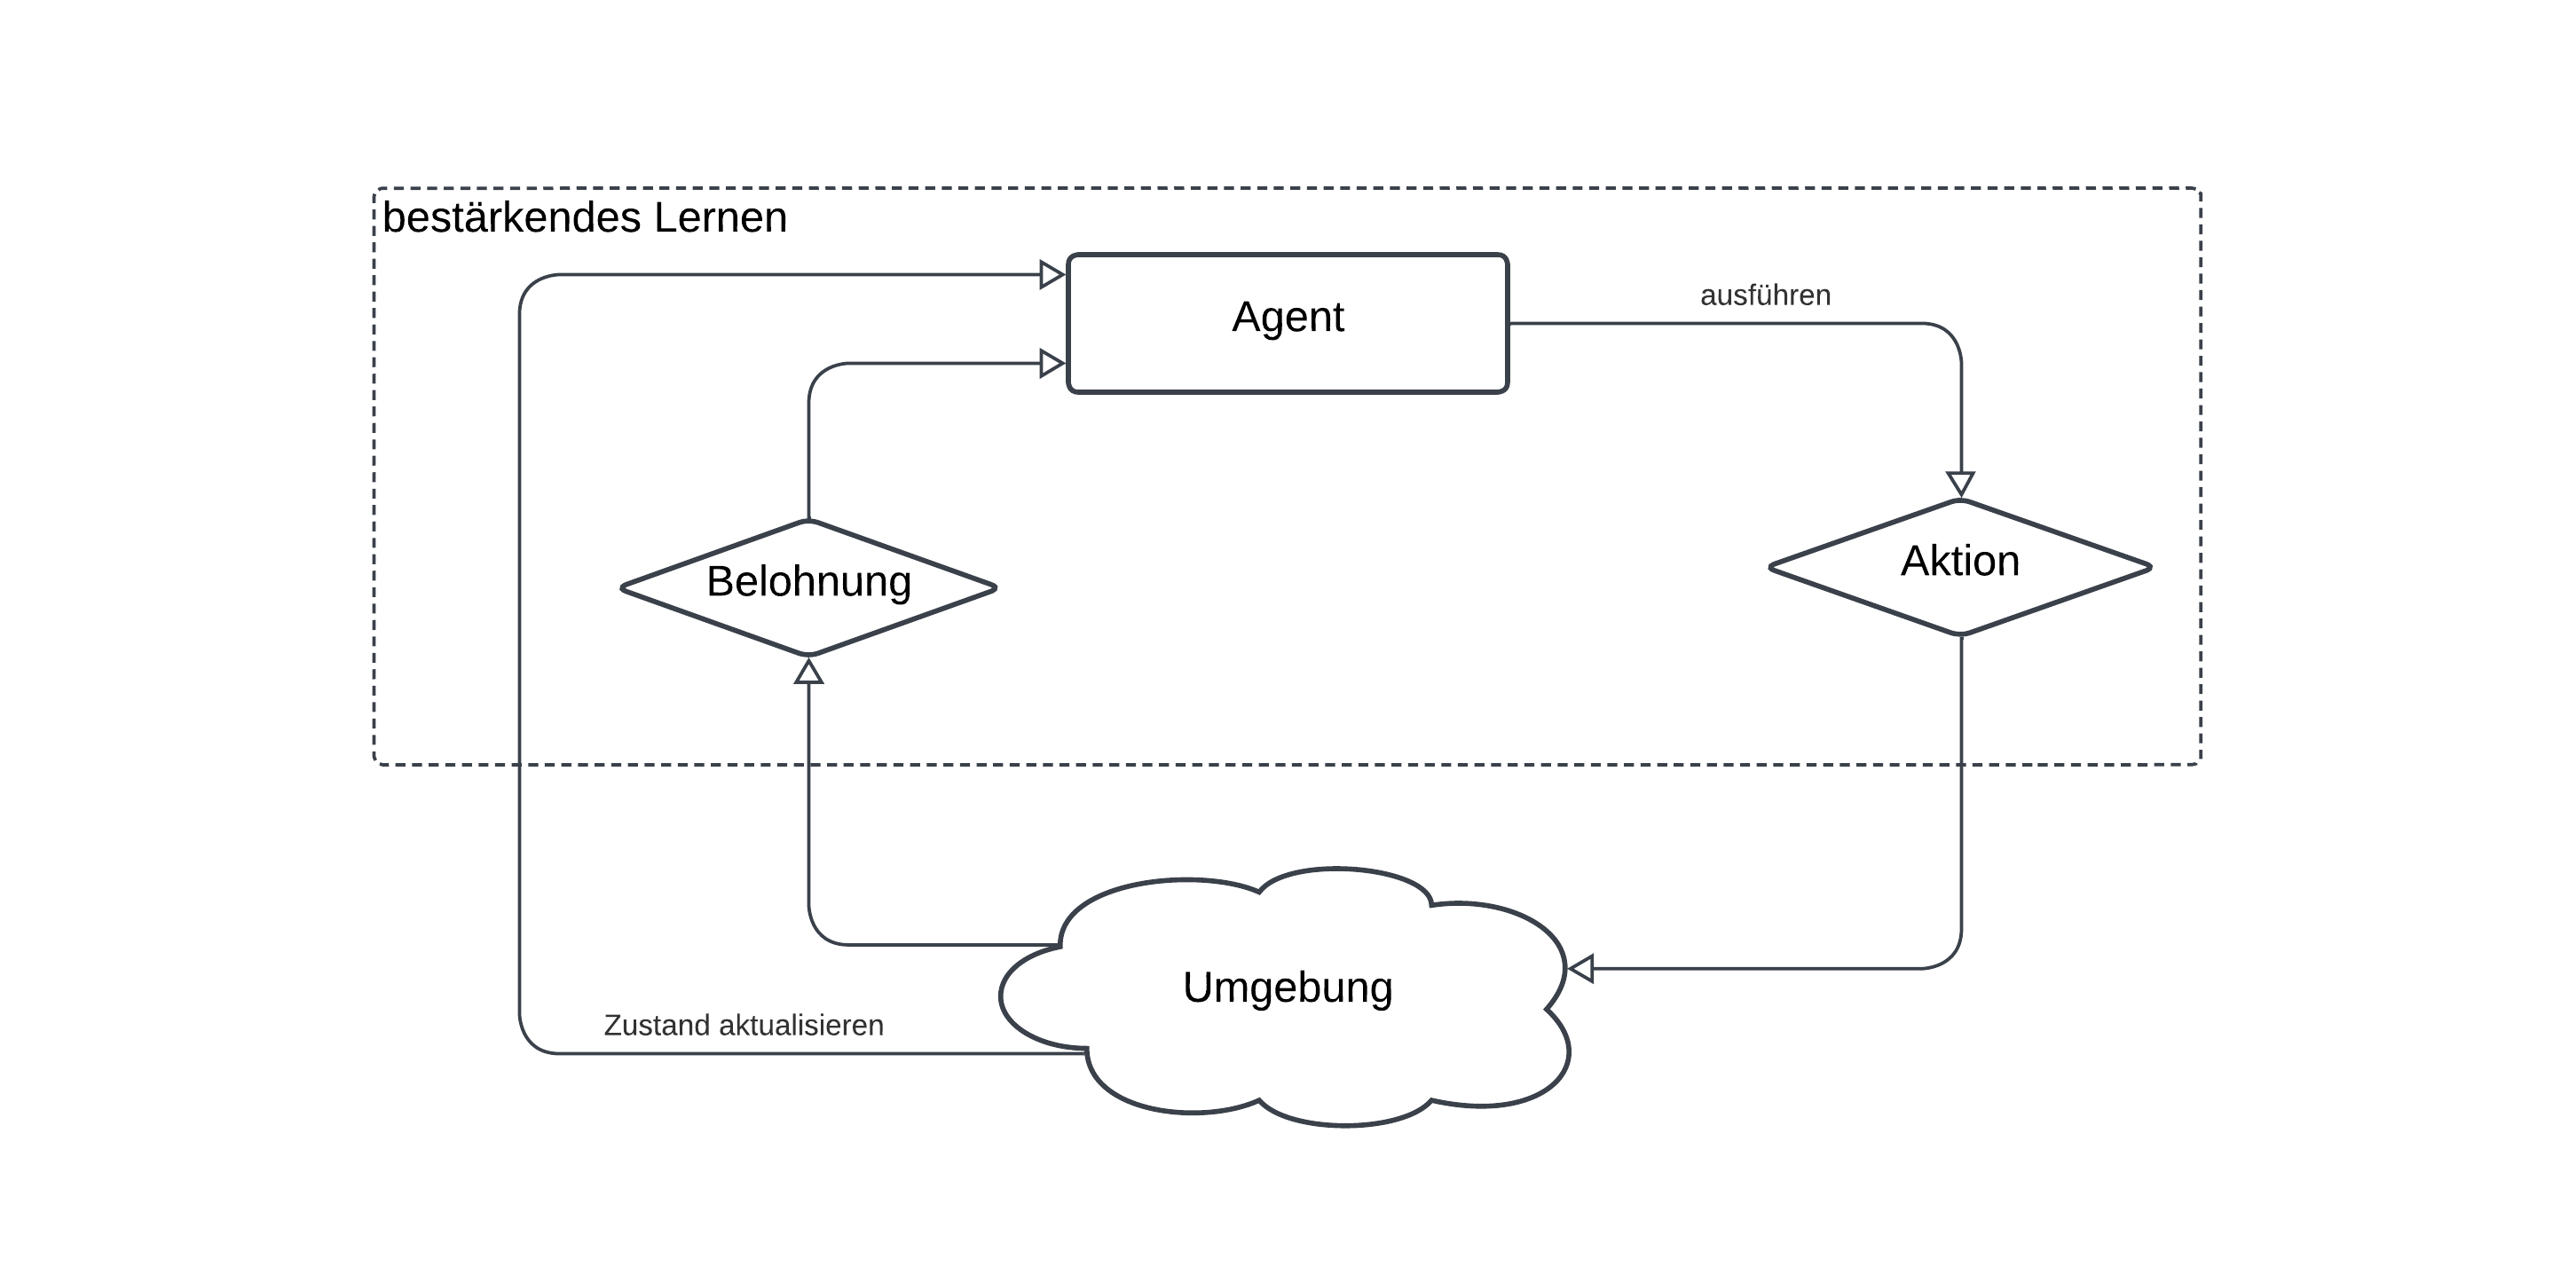
\includegraphics[width=\linewidth]{Bilder/ReinforcementLearning.png}
	\caption{Prozessvisualisierung: bestärkendes Lernen}
\end{figure}
Der \textit{Ablauf} des Trainings kann wie folgt beschrieben werden: Zu Beginn des Algorithmus setzt man die Parameter des Lernalgorithmus und des Agenten, wie Q-Werte, Policy und andere relevante Variablen auf einen bestimmten Startwert. Der Agent beobachtet hier den aktuellen Zustand der Umgebung mit einer bestimmten Methode (zum Beispiel visuell), um relevante Informationen für die Entscheidungsfindung aufzunehmen. Basierend auf seine interne Policy oder Schätzungen der Q-Werte des beobachteten Zustands der Umgebung wählt der Agent eine Aktion, um einen neuen Zustand herbeizuführen. Die Umgebung verändert ihren Zustand und gibt eine Belohnung, wie auch den neuen Zustand, an den Agenten zurück. Der Agent aktualisiert seine internen Modelle, um die Qualität seiner Entscheidungen zu verbessern, indem er den neuen Zustand analysiert und Belohnungen interpretiert. Beim Wählen der nächsten Aktion steht der Agent vor der Entscheidung der Exploration einer neuen Aktion und der Exploitation einer bereits durchgeführten. Der Prozess, beginnend mit der Auswahl einer bestimmten Aktion, wiederholt sich für eine gegebene Anzahl an Epochen beziehungsweise Schritten bis zur Konvergenz des Modells oder dem Erreichen einer akzeptablen Leistung.

Die Bewertung der \textit{Qualität} eines mit bestäkendem Lernen trainierten Modells stellt sich aufgrund der fehlenden Übertragbarkeit von traditionellen Metriken, wie Genauigkeit und Verlust, als komplexe Aufgabe dar. Eine Art der Leistungsbewertung kann mit Hilfe der kumulativen Belohnung sein, wobei ein höherer Wert darauf hindeutet, dass der Agent optimale Aktionen gelernt hat. Daneben kann man auch verschiedene andere Ansätze wie zum Beispiel Visualisierungen nutzen, um die Qualität eines Modells zu bewerten.